\chapter{Numerical Methods and Implementation}\label{ch:numerics}
The same control logic needs two numerical layers: evolution or precomputation of a policy, and feedback simulation of executions. We describe their accounting conventions first, then the inherited solver's limitations, the positive bounded-control scheme and physical-time export. C++ is an implementation of these mathematical operators, not an independent model or a separate empirical result.
\section{Simulation and Experimental Design}


\subsection{The Time-Discretized Simulation Engine}
To numerically evaluate the strategies' performance, a custom simulation engine was implemented in Python. Contrary to a purely time-discretized approach, which would be analytically complex when coupling continuous diffusion processes (mid-price) with discrete jump processes (market orders), the simulator relies on an Euler-Maruyama discretization scheme.

The time horizon $T$ is partitioned into $N$ equidistant intervals of length $\Delta t$. At each discrete time step $t_i$, given the state vector comprising the mid-price $S_{t_i}$, the accumulated inventory $q_{t_i}$, and the cash account $X_{t_i}$, the simulator executes the following logical cycle.

\begin{enumerate}
    \item \textbf{Quote Generation:} The active policy computes the optimal quote prices $p^{bid}$ and $p^{ask}$ based on the current state, the remaining time to horizon $\tau$, and the risk aversion parameter $\gamma$.
    \item \textbf{Probability Evaluation:} The theoretical Poisson intensities $\lambda^{bid}$ and $\lambda^{ask}$ are mapped into discrete transition probabilities for the interval $\Delta t$, defined as
    \begin{align*}
        p_{fill} = 1 - e^{-\lambda \Delta t}.
    \end{align*}
    \item \textbf{Execution Matching:} Two independent uniform random variables, $U^{bid}_{t_i}, U^{ask}_{t_i} \sim \mathcal{U}(0,1)$, are compared with the respective fill probabilities. If $U < p_{fill}$, the order is considered executed. In this implementation, each side can have at most one unit fill per time step and the rule is therefore a Bernoulli discretization of the underlying Poisson arrival process.
    \item \textbf{State Update:} In the event of a bid execution, inventory increases ($q_{t_{i+1}} = q_{t_i} + 1$) and the cash account decreases by the bid price ($X_{t_{i+1}} = X_{t_i} - p^{bid}$). Conversely, an execution at the ask reduces inventory and increases cash.
    \item \textbf{Mark-to-Market:} Performance is recorded by updating the total wealth (PnL), defined as
    \begin{align*}
        W_{t_{i+1}} = X_{t_{i+1}} + q_{t_{i+1}} S_{t_{i+1}}.
    \end{align*}
\end{enumerate}

\subsection{Experimental Control: Common Random Numbers (CRN)}
To rigorously isolate the performance differential between the symmetric benchmark and the inventory-aware policies, the experimental design employs the variance reduction technique known as Common Random Numbers (CRN).

In the Monte Carlo probability space, the entire stochastic scenario is pre-calculated via vectorized matrices. For each $m$-th simulated trajectory, a single master seed generates, at first, the sequence of Brownian increments ($\Delta W^{(m)}$) driving the mid-price process. Then the uniform random variables ($U^{bid, (m)}, U^{ask, (m)}$) governing order execution at each tick.

Both the Naive dealer and the Avellaneda--Stoikov dealer are tested on the exact same scenario. By subjecting the algorithms to the same price shocks and client order flows, the experimental design eliminates inter-path stochastic noise. Any observed disparity in terminal wealth or inventory accumulation is therefore solely attributable to the internal risk-management logic of the respective algorithms.

\subsection{Performance Metrics}
The simulator tracks the state variables to extract terminal distributions. Terminal wealth $W_T$ is reported on a mark-to-market basis, i.e., it includes the cash account plus the value of any remaining inventory at the terminal mid-price; no separate forced liquidation trade or liquidation cost is applied. The comparative analysis is based on the following key metrics:

\begin{itemize}
    \item Expected Terminal Wealth ($\mathbb{E}[W_T]$): the average profit generated across all Monte Carlo paths, representing the pure spread-capture capability.
    \item Wealth Variance ($Var(W_T)$): the dispersion of terminal PnL, acting as the primary proxy for unmanaged inventory and price risk.
    \item Sharpe-like ratio: calculated as the ratio between average terminal PnL and its standard deviation across Monte Carlo paths. It is an internal simulation diagnostic, not an annualized market Sharpe ratio.
    \item Expected Absolute Terminal Inventory ($\mathbb{E}[|q_T|]$): the average magnitude of the open position remaining at the end of the trading horizon $T$. This metric quantifies the strategy's capacity for mean-reversion, measuring how effectively it avoids overnight directional exposure.
    \item Inventory Dispersion ($\mathbb{E}[Std(q_t)]$): the average standard deviation of the inventory throughout the trading session. This metric captures the intraday risk profile, distinguishing between a strategy that tightly bounds its position (capital efficiency) and one that suffers large directional swings, regardless of the final terminal state.
    \item Expected Turnover ($\mathbb{E}[\text{Turnover}]$): the average volume of executed trades per simulation, serving as a proxy for the strategy's operational efficiency and its potential vulnerability to unmodeled transaction costs.
\end{itemize}

The analysis does not rely on the calibration of real historical data but rather on the definition of stylized scenarios. This approach allows for systematic stress-testing of the models in controlled regimes (varying volatility $\sigma$ and book density $k$), ensuring maximum reproducibility and isolating the structural mechanisms of the Avellaneda--Stoikov framework without the biases inherent to specific market datasets.





\subsection{Figure Construction Algorithms}
The numerical figures are produced from the same simulation objects used to compute the tables. To avoid repeating the same methodological explanation below each figure, we report the plotting logic once here as part of the simulation design. Panels (a)--(d) in the single-asset ABM and GBM figures follow the four algorithms below: mid-price and quotes, inventory path, mark-to-market PnL, and Monte Carlo terminal PnL distribution. In the multivariate figure, however, the first mid-price-and-quotes panel is intentionally not reported: we did not produce the multivariate mid-price-and-quotes graph because, with three assets, plotting all mid-prices together with their bid and ask quotes would make the panel unreadable. For this reason, panel (a) of the multivariate figure is replaced by cumulative log-returns, while panels (b)--(d) preserve the same portfolio-risk, PnL, and terminal-distribution logic.

\begin{algorithm}[H]
\caption{Panel (a): Mid-price and quotes}
\DontPrintSemicolon
\KwIn{Time grid $(t_i)_{i=0}^{n}$, simulated mid-price path $(S_{t_i})$, quoted bid and ask arrays for the naive and AS strategies.}
\KwOut{A price panel comparing the reference mid-price with the two quoting rules.}
Plot the mid-price path $S_{t_i}$ as the common reference line\;
Plot the naive bid and ask quotes $p_{t_i}^{bid,N}$ and $p_{t_i}^{ask,N}$ around $S_{t_i}$\;
Plot the AS bid and ask quotes $p_{t_i}^{bid,AS}$ and $p_{t_i}^{ask,AS}$ around the inventory-adjusted reservation price\;
Use the panel to visualize the quote skew: the naive quotes remain symmetric around $S_t$, while the AS quotes move with inventory through $r_t$\;
\end{algorithm}

\begin{algorithm}[H]
\caption{Panel (b): Inventory path}
\DontPrintSemicolon
\KwIn{Time grid $(t_i)_{i=0}^{n}$ and inventory paths $(q_{t_i}^{N})$, $(q_{t_i}^{AS})$.}
\KwOut{A pathwise comparison of inventory accumulation and mean-reversion.}
For each strategy, update inventory after bid and ask fills according to $dq_t=dN_t^{bid}-dN_t^{ask}$\;
Plot the naive inventory path $q_{t_i}^{N}$ and the AS inventory path $q_{t_i}^{AS}$\;
Add the zero-inventory line as the natural benchmark\;
Use the panel to evaluate whether the quoting rule creates an endogenous pull back toward $q_t=0$\;
\end{algorithm}

\begin{algorithm}[H]
\caption{Panel (c): Mark-to-market PnL}
\DontPrintSemicolon
\KwIn{Cash paths $(X_{t_i}^{N})$, $(X_{t_i}^{AS})$, inventories $(q_{t_i}^{N})$, $(q_{t_i}^{AS})$, and price path $(S_{t_i})$.}
\KwOut{A realized path of mark-to-market wealth for both strategies.}
At each time step, compute realized wealth as $W_{t_i}=X_{t_i}+q_{t_i}S_{t_i}$ in the single-asset case\;
For the multivariate case, compute $W_{t_i}=X_{t_i}+q_{t_i}^{\top}S_{t_i}$\;
Plot the naive and AS wealth paths on the same axes\;
Interpret the panel only as one realized scenario, not as the final statistical comparison\;
\end{algorithm}

\begin{algorithm}[H]
\caption{Panel (d): Terminal PnL distribution}
\DontPrintSemicolon
\KwIn{Monte Carlo samples of terminal wealth $\{W_T^{N,(m)}\}_{m=1}^{M}$ and $\{W_T^{AS,(m)}\}_{m=1}^{M}$.}
\KwOut{A density histogram comparing terminal PnL dispersion across strategies.}
Run both strategies on the same simulated price paths and fill uniforms using common random numbers\;
Collect terminal mark-to-market PnL $W_T^{(m)}$ for each Monte Carlo path $m=1,\ldots,M$\;
Build normalized histograms using the same bins for the naive and AS samples\;
Add vertical lines at the sample means of the two terminal PnL distributions\;
Use the panel to compare dispersion and tail exposure, not only average terminal PnL\;
\end{algorithm}

With the simulation architecture fixed, the remaining task is empirical comparison within the stylized Monte Carlo environment. The results chapter combines the diffusion diagnostics with the finite-lift and positive-baseline experiments under their separate accounting conventions.
\section{Inherited scalar audit and positive bounded baseline}


The audit imports the inspected HFT2 source without modifying it and runs its default scalar solver for $H=0.2$. Synthetic stationary lifted states are sampled with seed 42. Evaluation uses time indices $0$, $195$ and $388$, five inventory levels and twelve states per combination, producing 180 interior samples. Time differentiation is forward, spatial differences follow the inherited solver and derivative values are linearly interpolated.

\begin{center}
\begin{tabular}{@{}lr@{}}
\toprule
Diagnostic & Value \\
\midrule
Full aggregate instantaneous variance & $1.000000$ \\
Reduced diffusion variance & $0.209552$ \\
Full residual RMS & $138562.58$ \\
Reduced residual RMS & $113726.58$ \\
Operator-difference RMS & $38015.32$ \\
Pre-terminal entries at lower clip $-60$ & $6514$ \\
Pre-terminal entries at upper clip $15$ & $159144$ \\
\bottomrule
\end{tabular}
\end{center}

These unnormalized values are diagnostics under the declared discretization and bounded Hamiltonian. The inherited solver clips its value array and uses a different, unconstrained arrival term. Both choices matter when interpreting the residual. Entries at clipping bounds do not by themselves identify the cause of the numerical behavior, but the combination of extensive saturation and a large reduced residual rules out treating this run as a validated converged baseline. Its RMS magnitudes must not be directly ranked against the later positive-baseline off-grid diagnostic: sample sets, derivative reconstruction and numerical surfaces differ.

An independent C++ evaluation agrees with the exported Python residuals on all 180 samples within the prescribed relative tolerance $10^{-9}(1+|R|)$. The deterministic test executable passes 528 checks. These results verify implemented arithmetic and selected interfaces; they do not validate an optimal policy or justify a correction fit on the saturated baseline.

\section{A positive transformed baseline}
To address this issue, the next implementation uses $u=\exp(-\gamma\theta)>0$. On the scalar state grid its equation is
\begin{align*}
0={}&u_t+\mathcal L_Ru+\tfrac12\gamma^2q^2v(y)u\\
 &+\sum_{\pm}\min_{\delta\in[0.02,4]}
 Ae^{-k\delta}\bigl(e^{-\gamma\delta}u_{q\pm1}-u_q\bigr),
\end{align*}
where forbidden inventory transitions are omitted. The terminal condition is $u(T,q,y)=\exp(\gamma L(q,y))$. The transformation removes the spatial gradient-square term; it does not remove the coupled control optimization over neighboring inventories.

For spacing $h$, use nonnegative state-transition rates
\[
 a_-={\eta^2\over2h^2}+{\max(-b,0)\over h},\qquad
 a_+={\eta^2\over2h^2}+{\max(b,0)\over h},\qquad b=-\kappa y.
\]
Outward state transitions are suppressed at the two truncated boundaries. Each backward explicit step uses the minimizing quotes computed from the current positive array. The condition
\[
 \Delta t\left(a_-+a_++2Ae^{-k\delta_{\min}}\right)<1
\]
is sufficient for nonnegative coefficients in each controlled step; the inventory-risk term adds a nonnegative diagonal contribution. This gives an algebraic positivity property of the scheme. It is not a proof of convergence to the unbounded-domain HJB. Domain truncation, consistency, time error and policy error still require study.

The implementation chooses substeps from a conservative global bound with safety factor $0.8$. It reports a failure if a transformed value becomes nonpositive or nonfinite; no clipping of $\theta$ is used. Deterministic tests pass for a constant solution, an analytic no-arrival constant-volatility limit, inventory symmetry, positivity and invalid grids.

\begin{center}
\begin{tabular}{@{}rrrr@{}}
\toprule
State points & Time steps & $\theta(0,0,0)$ & $\theta(0,2,0)$\\
\midrule
61 & 2340 & 6.701053 & 6.367267\\
61 & 4680 & 6.699587 & 6.365723\\
121 & 2340 & 6.701135 & 6.367370\\
121 & 4680 & 6.699669 & 6.365826\\
241 & 2340 & 6.701176 & 6.367421\\
241 & 4680 & 6.699709 & 6.365878\\
\bottomrule
\end{tabular}
\end{center}
All six runs keep $u$ positive. With 4680 time steps, the change in $\theta(0,0,0)$ from 121 to 241 points is approximately $4.08\times10^{-5}$; halving the time step at 241 points changes it by approximately $1.47\times10^{-3}$. These are selected-point refinement diagnostics, not global error bounds. These initial runs exported only time-zero values. The following experiment extends the export to physical-time slices and examines joint domain/grid sensitivity; independent residual validation remains open.

\section{Time-dependent policies and domain sensitivity}
The next increment retains 41 physical-time slices, including both endpoints, from each backward solve. Nine configurations combine 81, 161 and 241 state nodes with symmetric domains of four, five and six stationary standard deviations. All use 9360 actual time steps. These are discretizations of the same scalar model, not nine market models or simulated trading sessions. The CSV export contains 772317 state-time-inventory records. An unavailable quoting side at an inventory limit is stored as missing, not as a zero offset.

Figure~\ref{hft3-fig:temporal-policy} shows the solved baseline at three times. The rows expose the approach to the liquidation condition; the columns distinguish the certainty equivalent from executable offsets. Inventory is discrete, so horizontal bands are expected. White boundary rows mark forbidden trades. The color scales are local to each panel. Near the terminal time, aggressive offsets can reach the declared lower bound; this is a control constraint, not clipping of the value function.

\begin{figure}[p]
\centering
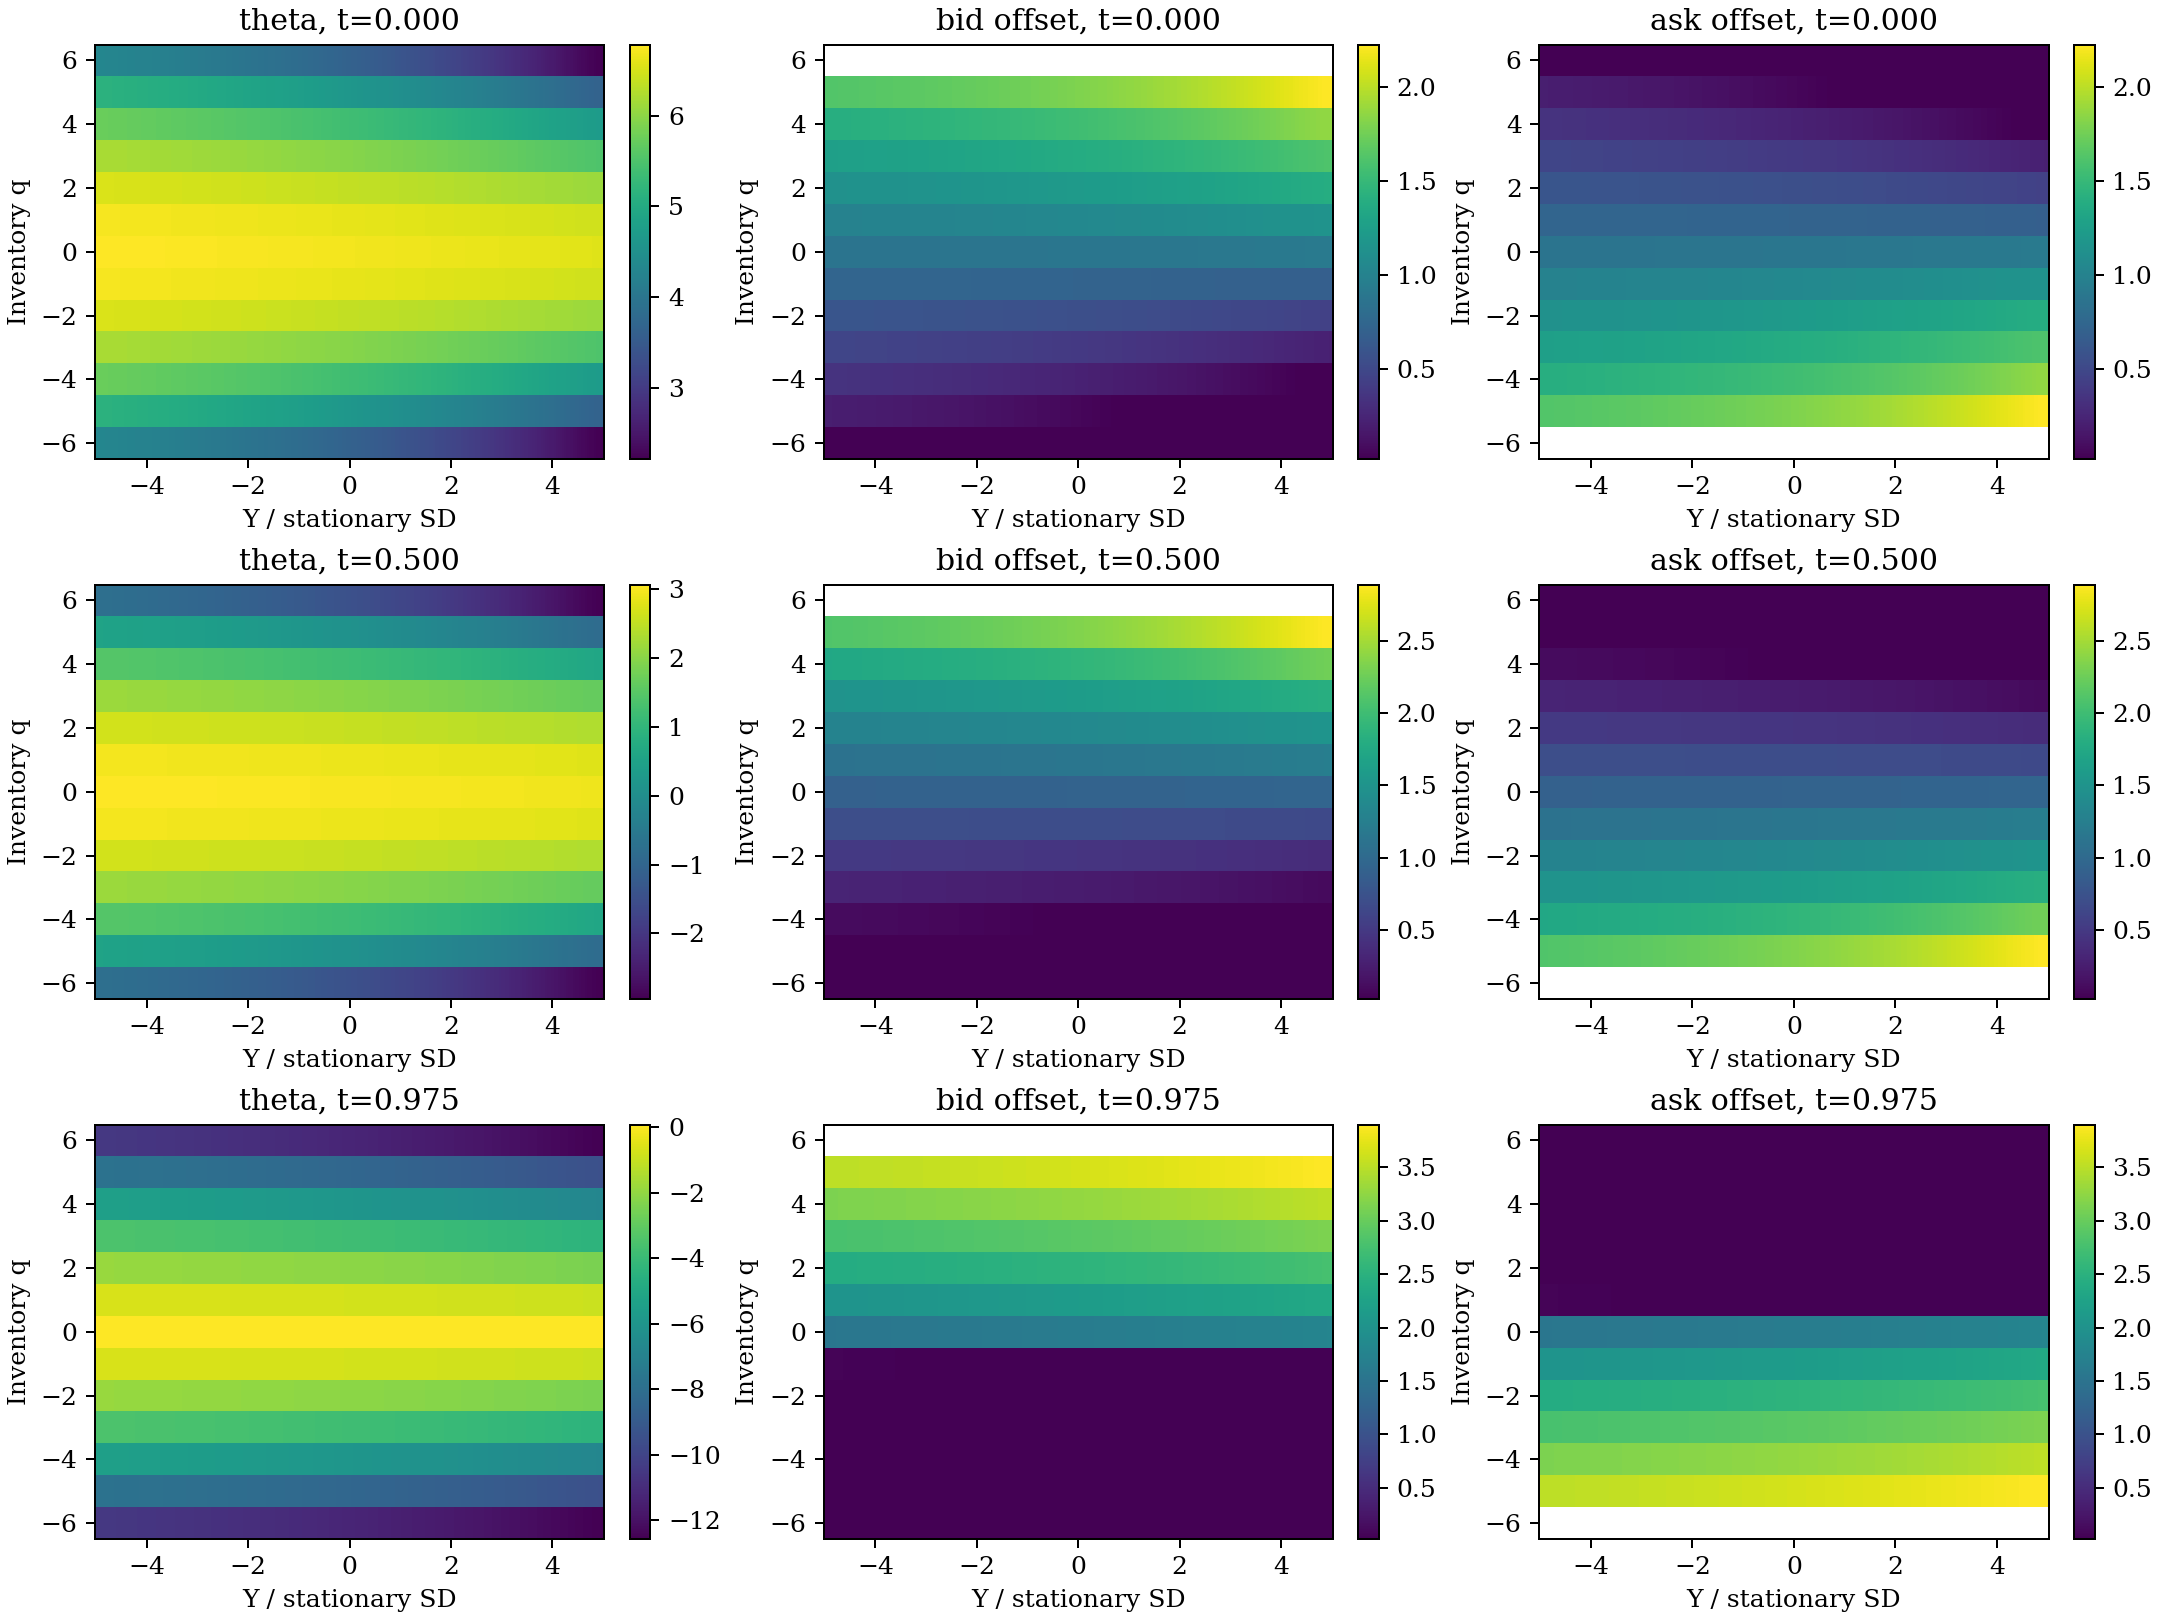
\includegraphics[width=\textwidth]{img/hft3-temporal_policy.png}
\caption{Solved scalar baseline: certainty equivalent and bid/ask offsets at $t=0$, $0.5$ and $0.975$, with $T=1$. Domain $\pm5$ stationary standard deviations, 241 state nodes, 9360 steps. Values and offsets use the model's monetary/price units; time is normalized. Blank cells denote disabled sides at inventory limits. Deterministic HJB computation, not Monte Carlo.}
\label{hft3-fig:temporal-policy}
\end{figure}

The export checks recover the terminal condition with maximum absolute error $5.33\times10^{-15}$, and all available offsets remain in $[0.02,4]$. Additional C++ tests verify temporal ordering, endpoint inclusion, the analytic no-arrival risk limit at every saved time, and exact agreement between the final snapshot and the existing time-zero API. Exporting the history does not change the numerical evolution.

Figure~\ref{hft3-fig:policy-sensitivity} compares all saved times, inventory levels and admissible sides on 101 common points in $|Y|\leq2\sqrt{\operatorname{Var}(Y)}$. Linear interpolation maps each grid to these points. The six-standard-deviation, 241-node run is a comparison surface, not an exact solution. Across the configurations, maximum differences are approximately $1.62\times10^{-3}$ for the value and $1.15\times10^{-3}$ for offsets. The zero at the reference configuration is an identity, not evidence of zero numerical error.

\begin{figure}[htbp]
\centering
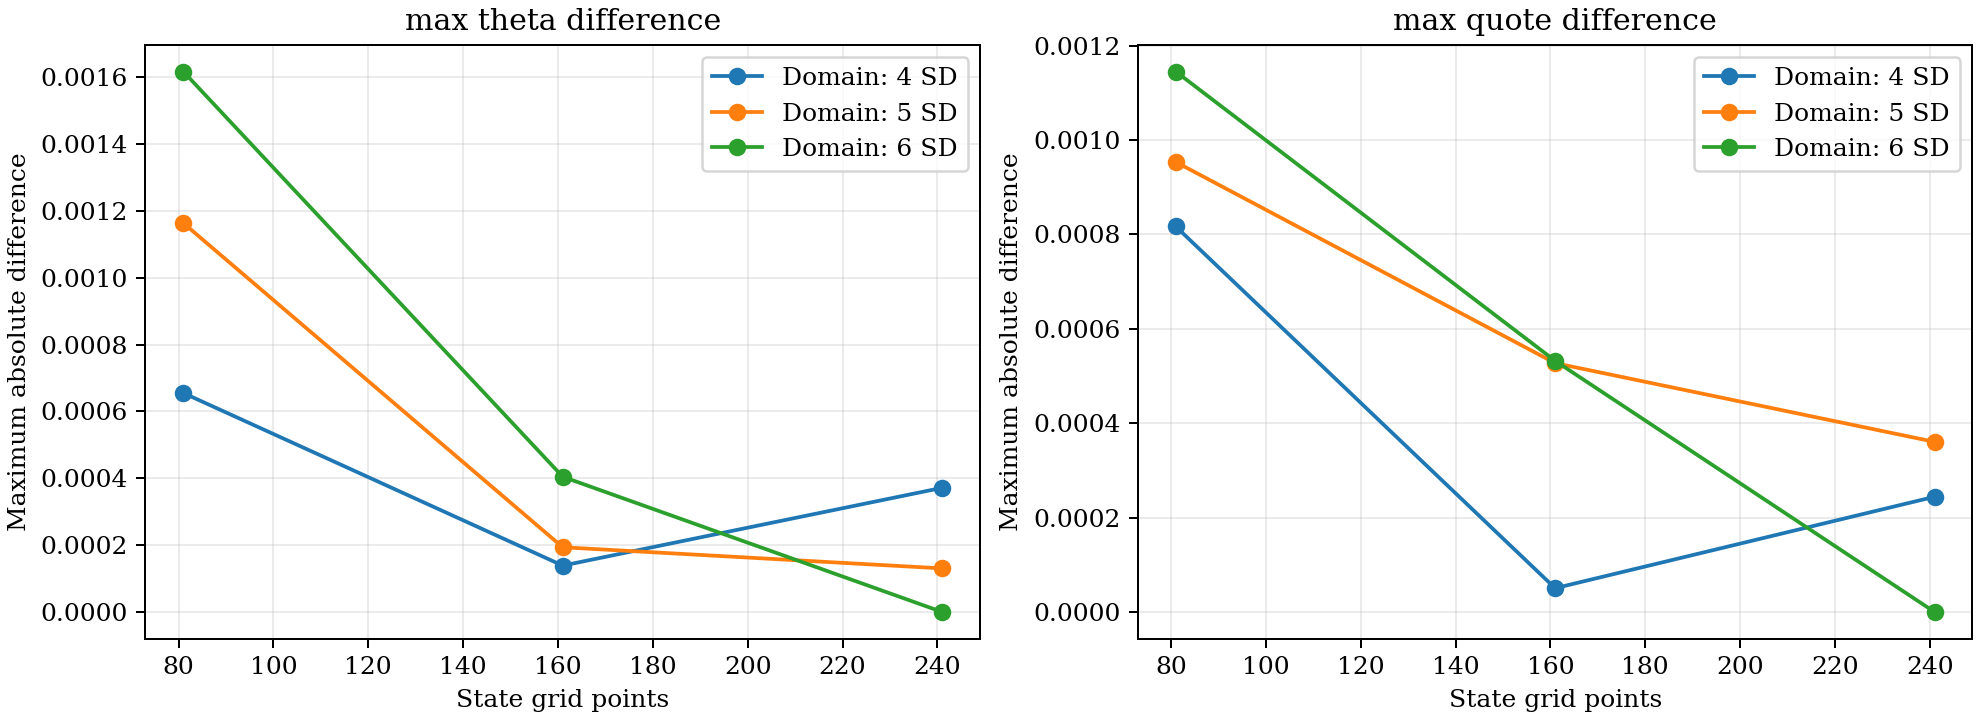
\includegraphics[width=\textwidth]{img/hft3-policy_sensitivity.png}
\caption{Joint grid/domain sensitivity relative to the six-standard-deviation, 241-node run, at a common 9360 time steps. Maxima cover all 41 saved times and the central two-standard-deviation interval. Changing the domain at fixed node count also changes spacing; the nonmonotone four-standard-deviation curve cannot be interpreted as an isolated boundary error.}
\label{hft3-fig:policy-sensitivity}
\end{figure}

The computational purpose of precomputation is to move HJB evolution outside the decision loop. Saving selected slices costs memory proportional to the number of stored times, inventory levels and state nodes, rather than requiring every solver step to be retained. This increment supplies offline CSV data; interpolation refinement and a measured speed advantage remain pending. The separate temporal and fixed-spacing studies reported in the comparative-results chapter extend these joint sensitivities; independent derivative/residual convergence remains a gate before fitting corrections. In particular, the figures do not yet establish full-state accuracy or economic performance.

\clearpage
\section{C++ operators and offline policy export}


The implemented offline path evaluates the full operator and exports baseline policy surfaces; fitting corrections remains a proposed extension. The online target is a fixed-size factor update, aggregation, baseline lookup, gate evaluation and a small bounded number of correction lookups. The state recurrence alone costs $O(M)$. Exact correlated OU innovation generation with a dense precomputed factor costs $O(M^2)$ per simulation step; its factorization costs $O(M^3)$ offline. Correction cost also includes feature construction and support selection. These components must be timed separately before assigning a complexity or latency to the complete decision. The offline Hessian contraction currently costs $O(M^2)$; it is not part of the online latency claim.

The first implementation provides a bounded arrival Hamiltonian, a common-noise full residual evaluator, scalar-to-vector derivative embedding, a smooth gate and exact correction-product derivatives. Parameters and diagnostic inputs are validated. Arithmetic overflow in the residual is reported instead of silently clipping it. Tests cover inventory limits, quote optimization against a grid search, mixed Hessian terms, scalar embedding, gate derivatives and nonlinear recomputation.

The archived original demonstration used synthetic surfaces without a time coordinate. A finite-horizon solved policy must represent the remaining time explicitly or use an equivalent validated selection of time slices. It would be misleading to report the starter's lookup as the performance of the future corrected HJB policy.

Software timing will be measured separately for factor updates, baseline lookups, corrections and the complete decision. Warm-up, timer overhead, repeated trials, compiler flags and hardware disclosure are prerequisites. No exchange round-trip claim follows from a local microbenchmark. The comparative-results chapter reports the checks and experiments completed under these conventions.

The comparative-results chapter now applies these conventions to the diffusion models, memory-inspired finite lifts and covariance proxy. The mathematical form of a quote is shared, but terminal accounting, approximation level and numerical resolution are stated separately for each experiment.
